\section{Redes Neuronais \label{se:resml}}

Os vários métodos percorreram com muitos modelos, aqui apresento apenas os melhores baseados em GPD Positivo da experiência toda.\par


\begin{table}[H]
    \caption{Resultados métricas Modelos Neuronais}    
    \resizebox{\linewidth}{!}{\begin{tabular}{llrrrrrrrrr}
\toprule
 &  & RMSE & SAE & AllocF & AllocD & GPD & GPD F & GPD D & GPD norm & GPD Positivo \\
 & Arquitetura &  &  &  &  &  &  &  &  &  \\
\midrule
\multirow[t]{5}{*}{Alocação a Subir} & UNET200 & 317.86 & 9759154.87 & 151181.25 & 9607973.62 & 43.78 & 0.98 & 44.16 & 22.57 & 43.78 \\
 & VanillaCNN200 & 328.88 & 10208138.49 & 147549.10 & 10060589.40 & 41.19 & 3.36 & 41.53 & 22.44 & 41.19 \\
 & UNET & 349.91 & 11008787.25 & 146742.39 & 10862044.86 & 36.58 & 3.89 & 36.87 & 20.38 & 36.58 \\
 & VanillaCNN & 370.73 & 11804382.23 & 149719.91 & 11654662.32 & 31.99 & 1.94 & 32.26 & 17.10 & 31.99 \\
 & 2StackedCNN200 & 410.28 & 13223932.55 & 126341.23 & 13097591.32 & 23.82 & 17.25 & 23.87 & 20.56 & 23.82 \\
\cline{1-11}
\multirow[t]{5}{*}{Alocação a Descer} & UNET200 & 282.52 & 8243468.87 & 469060.52 & 7774408.35 & 36.50 & 2.11 & 37.82 & 19.97 & 36.50 \\
 & VanillaCNN200 & 289.59 & 8671975.58 & 476040.73 & 8195934.85 & 33.20 & 0.66 & 34.45 & 17.55 & 33.20 \\
 & UNET & 304.28 & 9172373.23 & 470149.87 & 8702223.36 & 29.34 & 1.89 & 30.40 & 16.14 & 29.34 \\
 & VanillaCNN & 313.42 & 9483287.93 & 475881.60 & 9007406.33 & 26.95 & 0.69 & 27.95 & 14.32 & 26.95 \\
 & VanillaFCNN200 & 344.05 & 10438899.42 & 476740.17 & 9962159.25 & 19.59 & 0.51 & 20.32 & 10.41 & 19.59 \\
\cline{1-11}
\bottomrule
\end{tabular}
}
    \label{tab:mlresmetrics}
    \end{table}

O melhor modelo para alocação a Descer apresenta um ganho de desempenho em relação ao benchmark de 33\%, e o a Subir de 43\% na soma da janela temporal de validação.\par
Estes modelos têm ambas as alocações e os erros menores que o benchmark. Considerando que os dados que permitem quantificar a mais valia económica de reduzir a alocação de reserva secundária em falta devido não são dados públicos, o objetivo passa por manter esta alocações com valores mais baixos que o benchmark (GPDF positivo mas próximo de 0) e minimizar a alocação em excesso, maximizando o GPDD, ou juntando as condições maximizando o GPD Positivo. Desta forma a primeira arquitetura de cada tabela é aquela que apresenta melhores resultados quantificáveis quer do ponto de vista operacional como económico.\par
Escolhendo o modelo com melhores resultados em GPD Positivo podemos ver algumas janelas temporais.\par


\begin{figure}[H]
    \centering
    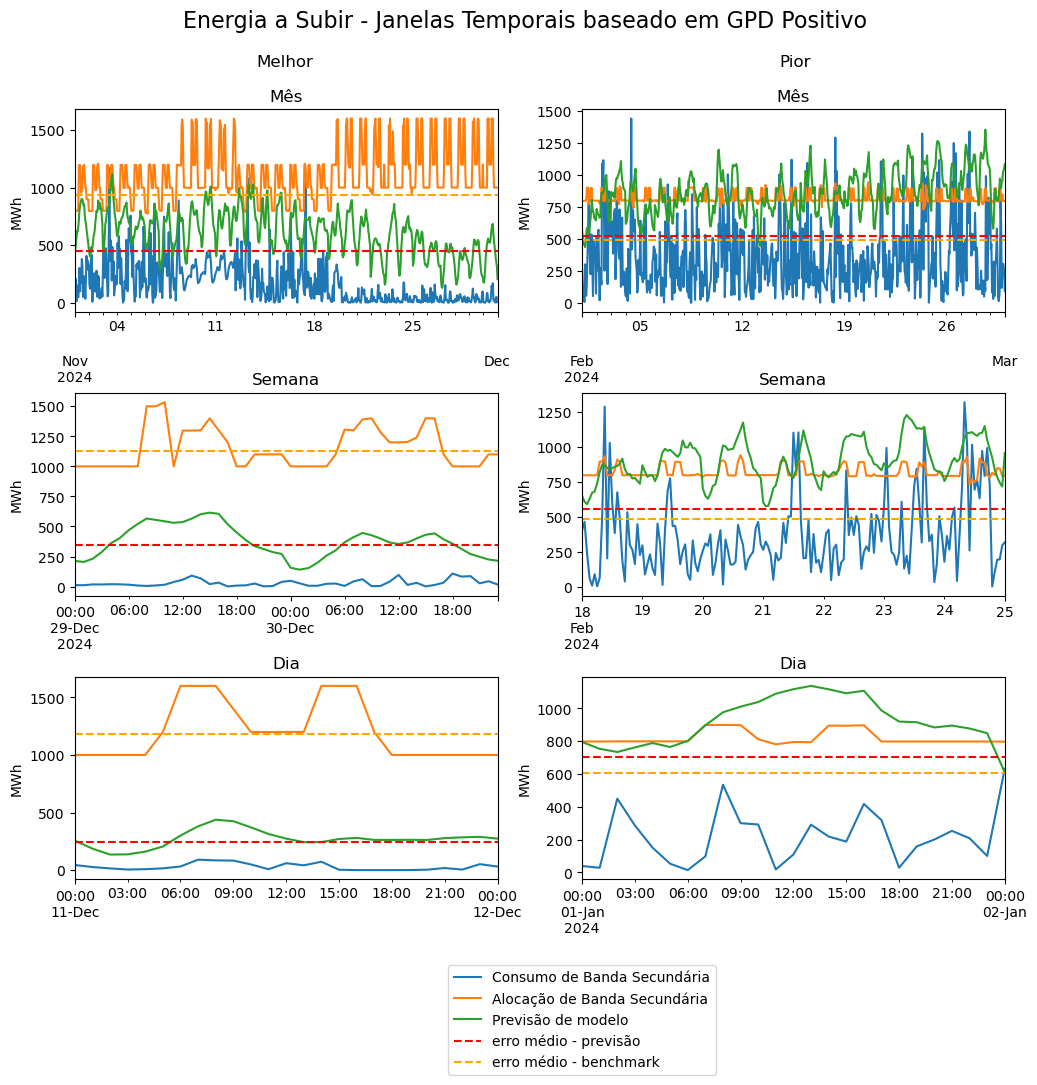
\includegraphics[width=\textwidth]{plots/alocacoes_temporais_upward_prediction_gpd_p.png}
    \caption{Janelas temporais energia a subir}
    \label{fig:mltimewindowsup}
\end{figure}


\begin{figure}[H]
    \centering
    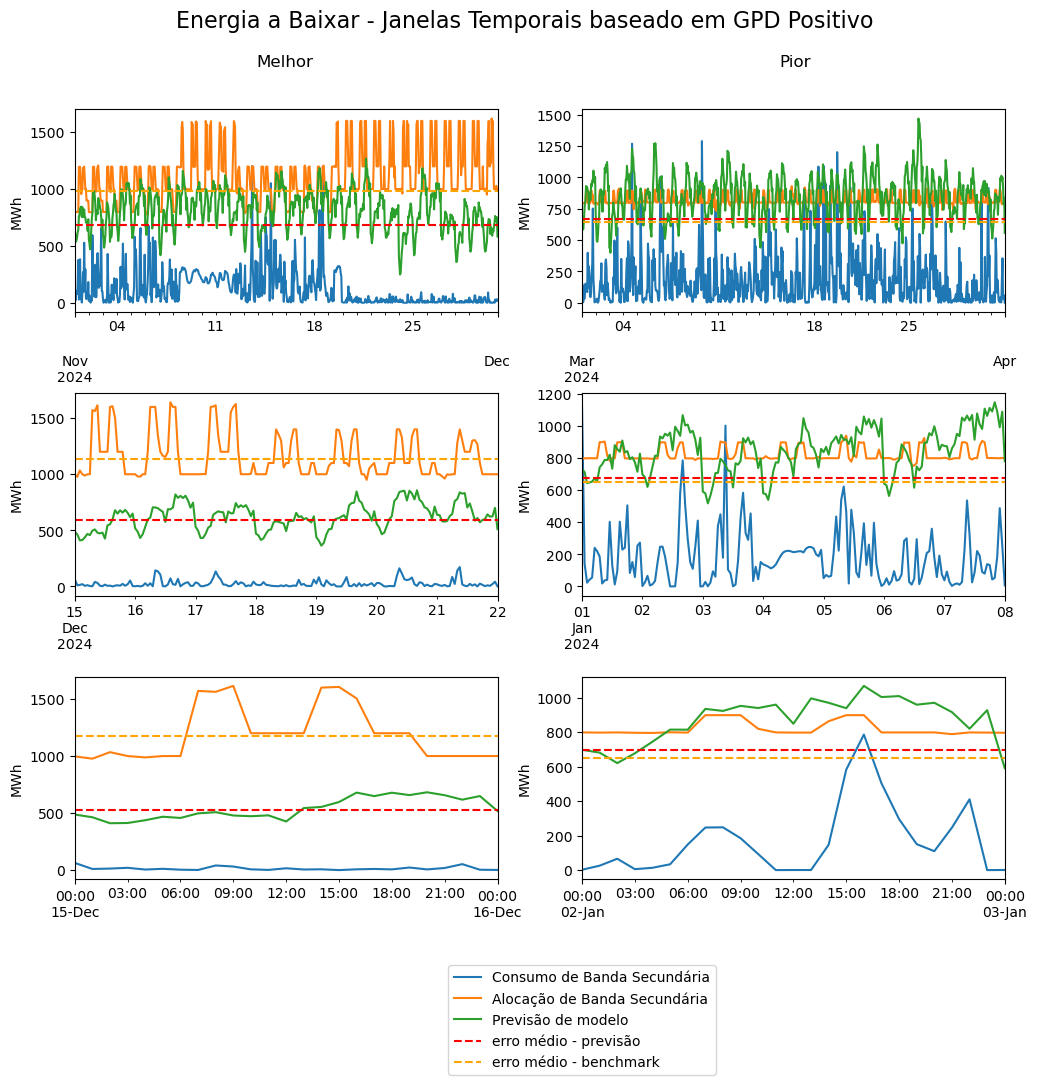
\includegraphics[width=\textwidth]{plots/alocacoes_temporais_downward_prediction_gpd_p.png}
    \caption{Janelas temporais energia a descer}
    \label{fig:mltimewindowsdown}
\end{figure}

Aqui é visualmente notável que o modelo mantém uma previsão mais perto da energia usada do que o benchmark. Mesmo nas piores janelas temporais, o erro de previsão acumulado é claramente menor que o do método actual.\par
Quero dar destaque também ao facto de as previsões seguirem bastante mais fielmente as curvas e picos apresentados. Especialmente nas janelas de mês onde temos mais amostras, conseguimos perceber que o modelo quase sempre acompanha picos da energia usada voltado a baixar quando estes passam. destacando-se assim do actual método que mantém uma linha de base bastante mais elevada (desperdiçando mais recursos) e com flutuações que não descrevem tão bem o real.\par
Esta flexibilidade no modelo de redes neuronais permite ao operador ter um sinal muito mais flexível diminuindo a alocação desperdiçada.\par

\begin{figure}[H]
    \centering
    \includegraphics[width=\textwidth]{plots/alocation_sum_over_time.png}
    \caption{Soma de Banda Secundária}
    \label{fig:mltimewindowssum}
\end{figure}

Os gráficos anteriores vêm rectificar esta mesma ideia, olhando para a Energia cumulativa dentro janelas em destaques vemos que o método proposto mantém quase sempre uma melhoria ao método utilizado. Mesmo quando passamos a janelas diárias e semanais embora aumente consideravelmente as vezes que o método proposto não é o melhor que o actual, mantém-se a premissa. E mais importante, o desenho das flutuações é bastante mais fiel ao real.\par


\begin{table}[H]
    \caption{Resultados Modelos}    
    \resizebox{\linewidth}{!}{\begin{table}[H] 
    \caption{Model Results and (allocated) values wthin 2024.\label{model_vs_bench}}
    \begin{adjustwidth}{-\extralength}{0cm}
    \newcolumntype{C}{>{\centering\arraybackslash}X}
    \begin{tabularx}{\fulllength}{CCCCCC}
    \toprule
    & & \textbf{mean}	& \textbf{std}	& \textbf{min} & \textbf{max}\\


    \midrule
            \multirow[m]{2}{*}{Down Allocation (MW)}	        & & (921.84) & (191.03) & (720.00) & (1708.00) \\
                                                                & & 836.85 & 182.04 & 247.82 & 1469.62 \\
            \multirow[m]{2}{*}{Up Allocation (MW)}	            & & (921.49) & (191.72) & (719.00) & (1694.00) \\
                                                                & & 778.42 & 228.85 & -29.47 & 1458.01 \\
            \multirow[m]{2}{*}{Hourly Capacity (MW)}	        & & (1843.32) & (382.35) & (1439.00) & (3399.00) \\
                                                                & & 1615.27 & 346.50 & 393.85 & 2594.85 \\
            \multirow[m]{2}{*}{Extraordinary Down Energy (MWh)}	& & (168.74) & (175.69) & (0.90) & (1214.00) \\
                                                                & & 149.66 & 179.96 & 2.66 & 1358.81 \\   
            \multirow[m]{2}{*}{Extraordinary Up Energy (MWh)}	& & (179.39) & (163.94) & (1.00) & (1054.80) \\
                                                                & & 141.85 & 153.57 & 1.83 & 1420.22 \\
    \bottomrule
    \end{tabularx}
    \end{adjustwidth}
\end{table}
}
    \label{tab:mlres}
    \end{table}



\begin{table}[H]
    \caption{$\Delta$\% das médias dos Modelos}    
    \resizebox{\linewidth}{!}{\begin{table}[H] 
    \caption{Mean $\Delta$\% between model and benchmark\label{model_vs_bench_perc}}
    \newcolumntype{C}{>{\centering\arraybackslash}X}
    \begin{tabularx}{\textwidth}{CC}
    \toprule
    & \textbf{$\Delta$\%} \\
    

    \midrule
            Down Allocation (MW)	        & -28.62 \\
            Up Allocation (MW)              & -37.26 \\
            Hourly Capacity (MW)	        & -33.24 \\
            Extraordinary Down Energy (MWh)	& -51.62 \\
            Extraordinary Up Energy (MWh)	& -59.47 \\
    \bottomrule
    \end{tabularx}
    % \noindent{\footnotesize{\textsuperscript{1} Tables may have a footer.}}
\end{table}


}
    \label{tab:mlres_deltas}
    \end{table}

O método proposto apresenta uma melhoria total de \textasciitilde44\% na alocação a subir e \textasciitilde37\% na alocação a descer face ao método usado no mercado. As melhorias médias são de \textasciitilde35\% e \textasciitilde25\% respectivamente, o que também é uma melhoria face ao estado da arte \cite{Algarvio2024} com 13\% e 8\%.\par
Libertando em média 30\% dos recursos horários, e baixando a necessidade de activar a reserva terciária em 45\% e 53\%.\par

As correlações entre o modelo e real são também mais elevadas que entre \hyperref[fig:featurecorrelation]{modelo e benchmark}.


\begin{figure}[H]
    \centering
    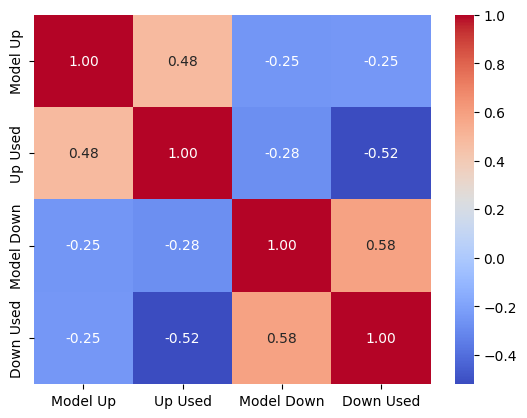
\includegraphics[width=\textwidth]{plots/heatmap_correlation_pred.png}
    \caption{Correlação entre previsão e real}
    \label{fig:predcorrelation}
  \end{figure}

Este mapa de correlações é quase o oposto do apresentado pelo \hyperref[fig:benchmarkcorr]{benchmark}.\par
Aqui as correlações maiores são, como seria de esperar, entre a energia usada e a sua alocaçao. Com 46\% na energia a subir e 55\% a descer. E as energias alocadas têm uma correlaçao baixa.\par 